\chapter{Results} \label{ch:results} % 13102 characters

\section{IPython notebook} % 4500 characters
The original python code was transferred to .ipynb notebooks.
This is the inner format of the Jupyther environment.
The notebook allows running the code in separate cells.
The cells can also contain markdown code for easier documentation.
Since not all part was required from the original code, only the required parts were transferred.

The main function (\cref{code:original}) of the algorithm is calling the separate functions of the other parts.
it can be seen on the 23rd line, the connection is established to the simulator server (\cref{code:client}).
The parameter 'veihcle=car' is just a setting option by the original designer.
The car profile was used for testing purposes, but the visual display of the vehicle was changed to the drone.
As the connection is established, the image is converted to an OpenCV image format (line 31).
This conversion is a built-in function of the airsim.
There is also an offline load function, however, it works only if the code is reworked, since the offline image should not be decoded (line 31), nor reshaped (line 34).

After loading the image the preprocess function (\cref{code:python_preproc}) selects the bounding boxes and passes it to the neural network (\cref{code:net}).
The most prominent bounding box is selected ('max\_index').
On the PYNQ system, there was no chainer library installed for previously described reasons, the neural network part was temporarily removed from the code.
This also prevented the system to select the max\_index item.
For that, the bounding boxes are drawn to all object detected by the preprocessing.
This is a better solution for validating the FPGA implementation since the input of the neural network can be directly observed, there is no need to speculate about abstract representations.
At the end of the code (line 62-65), the imshow line is updated to a matplotlib implementation because the cv2.imshow opens a new window, which operation is prevented by the PYNQ.
There is also an option for saving the image to the SD card for later analysis (line 67).

The client code is kept simple since the control of the drone is not yet the purpose of the system.
The basic settings (angle of arrival, travel height) can be set in the simulator before the start.
The main functions are the built-in python \_\_init\_\_, pause, and reset of the simulation and of course the get\_image.
As it can be seen inline 25, the function gets parameters of which camera to use, and which type of image to return.
The cameras on the vehicle can be accessed by following names in API calls: front\_center, front\_right, front\_left, fpv and back\_center. Here FPV camera is the driver's head position in the car.
For backward compatibility, you can still use following ID numbers for above camera names in the same order as above: "0", "1", "2", "3", "4".
In this system, the default camera is set to "1", which is the front\_right camera.
and the typ=0 is the 'Scene' camera which returns a regular RGBA image of the scene.

The client has another important function which may be discussed separately (\cref{code:training_data}).
This function is responsible for saving data to train the neural network.
The function requests two images at once from the simulator (line 4).
The first image is the regular scene image, and the other is a segmented one.
The segmented image is done by the airsim and returns the different area of the pictures.
The areas are represented by different colours based on the object type.
The segmented image than searched for contours (line 22).
The most prominent 4 boxes then added to the image and returning both the scene image and the bounding box as well.
With this, the neural network has the training set.
The preprocessed images are fed to the neural network and the network decides one of the boxes.
The decision should match up with the training bounding box.
It is easy to generate a big training data with all the different angles.

The neural network is a simple chainer CNN implementation.
There only two convolutional layers, and two fully connected one.
All the layers are applied to a ReLU function (line 34-38), and after the convolution, there is a max-pooling applied as well.
The first convolutional layer contains 10 output layers (line 23), and the second one contains 5 (line 24).
The two fully connected layers have 128 and 2 output layers. 

The preprocessing function takes an OpenCV image.
At first, it detects the horizon.
For this, it takes a series of numbers (line 2).
These points become the inflexion point of the segmented line of the horizon borderline.
Based on the complexity of the horizon (how segmented the line should be) not all the points are used.
After applying the horizon detect, comes the image processing part in question.
There is a series of OpenCV functions applied to the image (line 49-54).
There is an adaptive threshold function is replaced by a regular threshold function.
This was a necessity due the xfOpenCV does not have the adaptive threshold function implemented.
For the final result, both functions provide similar results, thus the two functions are interchangeable (\cref{fig:thresh_compar}).
There was also an attempt to implement the adaptive threshold for FPGA, but at the validation, the error measure was usually over 1\% which is too high error rate for an image processing system.
The final step is to find the contours on the image.
However, this part cannot be included in the FPGA system since there is a double cycle that manipulates the image, thus ruining the dataflow.

\begin{figure}
    \centering
    \begin{tabular}{ccc}
        
    % 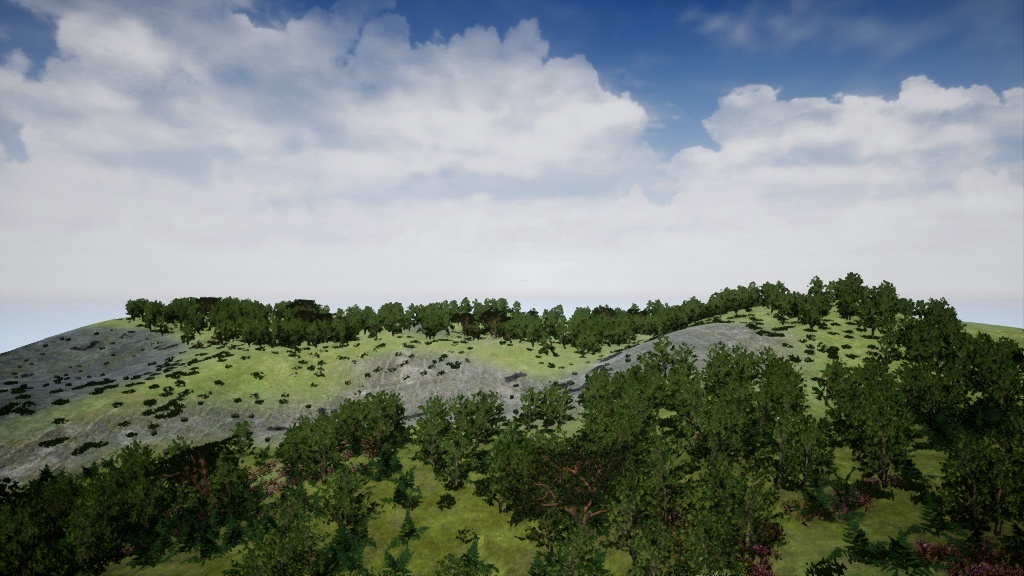
\includegraphics[width=.27\linewidth]{images/airsim_thresh/img_1.jpg} &
    % 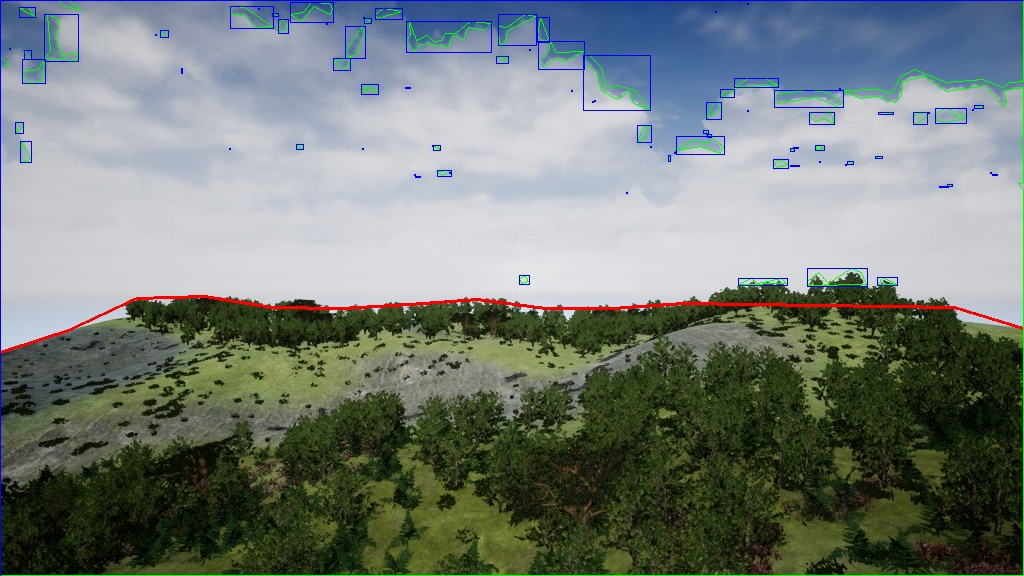
\includegraphics[width=.27\linewidth]{images/airsim_thresh/img_adaptive_1.jpg} &
    % 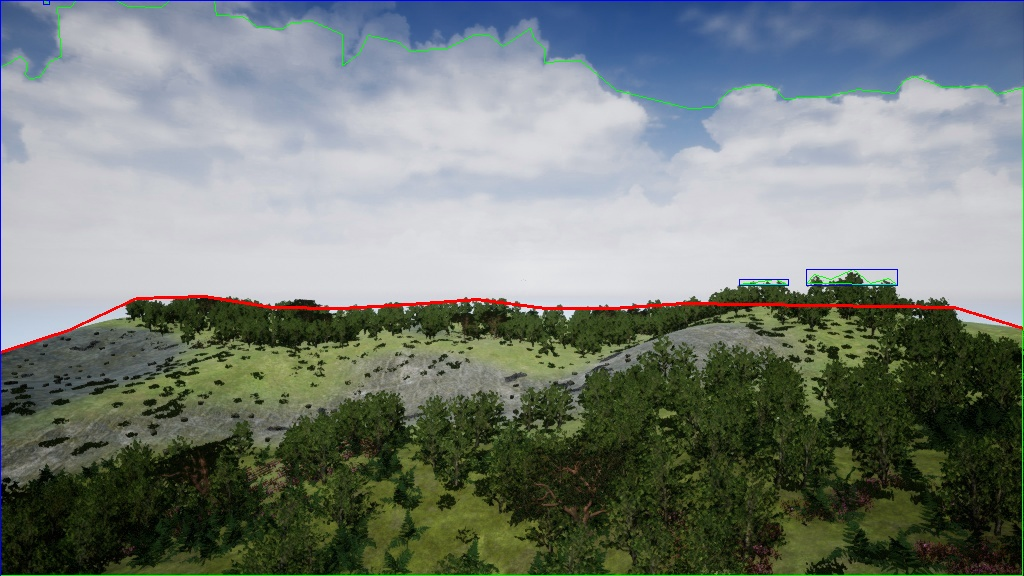
\includegraphics[width=.27\linewidth]{images/airsim_thresh/img_thresh_1.jpg} \\
    
    % 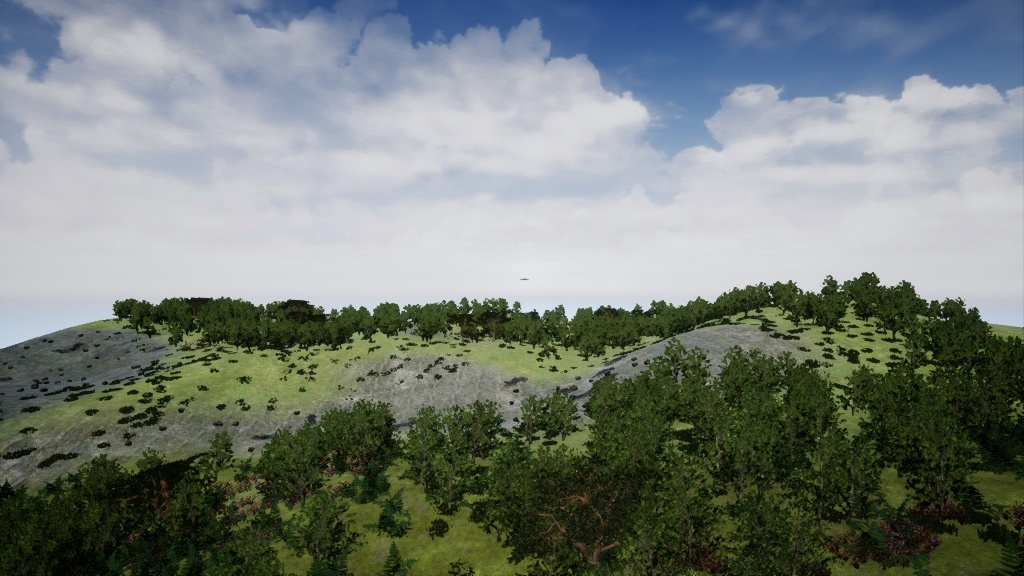
\includegraphics[width=.27\linewidth]{images/airsim_thresh/img_2.jpg} &
    % 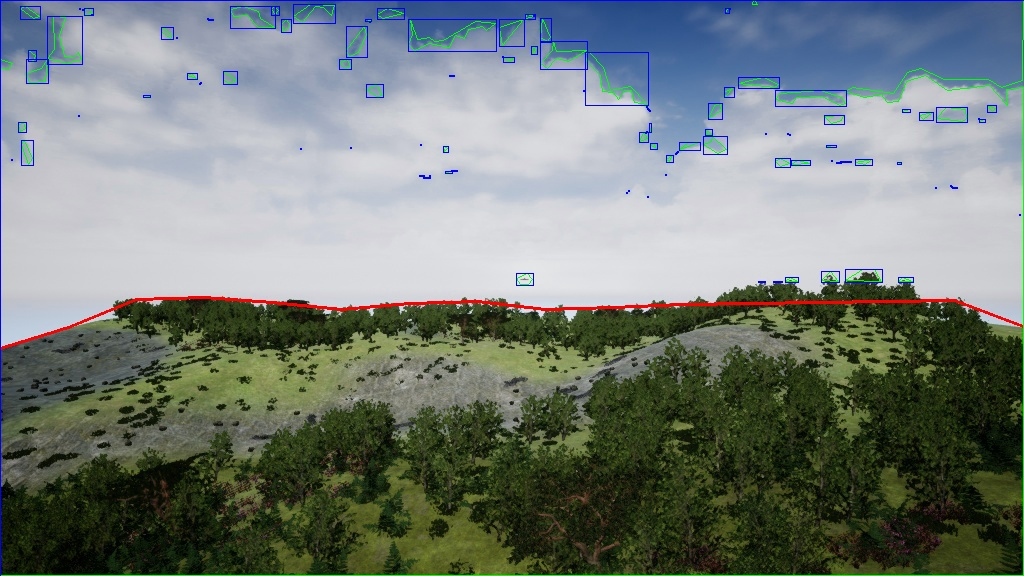
\includegraphics[width=.27\linewidth]{images/airsim_thresh/img_adaptive_2.jpg} &
    % 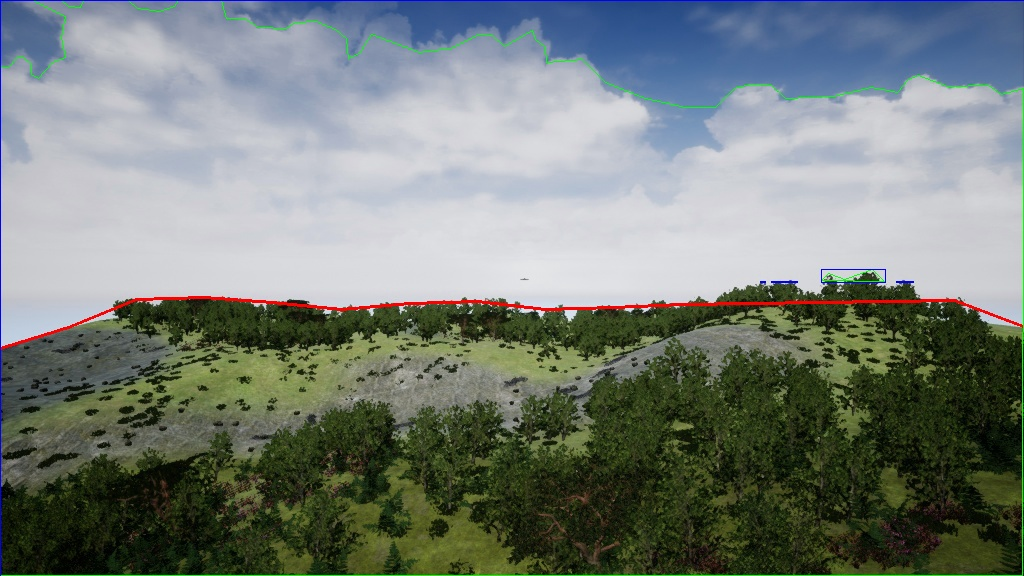
\includegraphics[width=.27\linewidth]{images/airsim_thresh/img_thresh_2.jpg} \\
    
    % 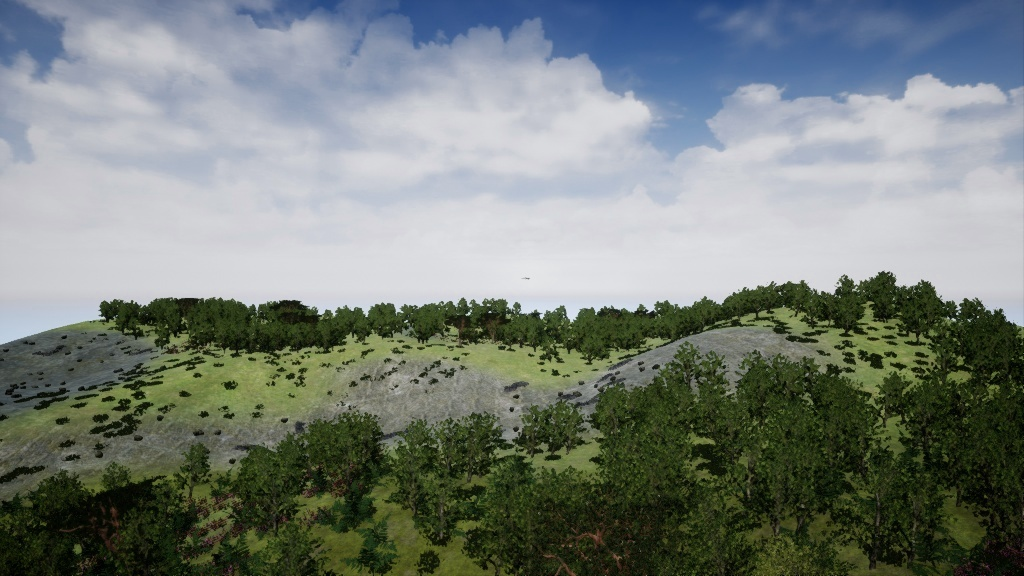
\includegraphics[width=.27\linewidth]{images/airsim_thresh/img_3.jpg} &
    % 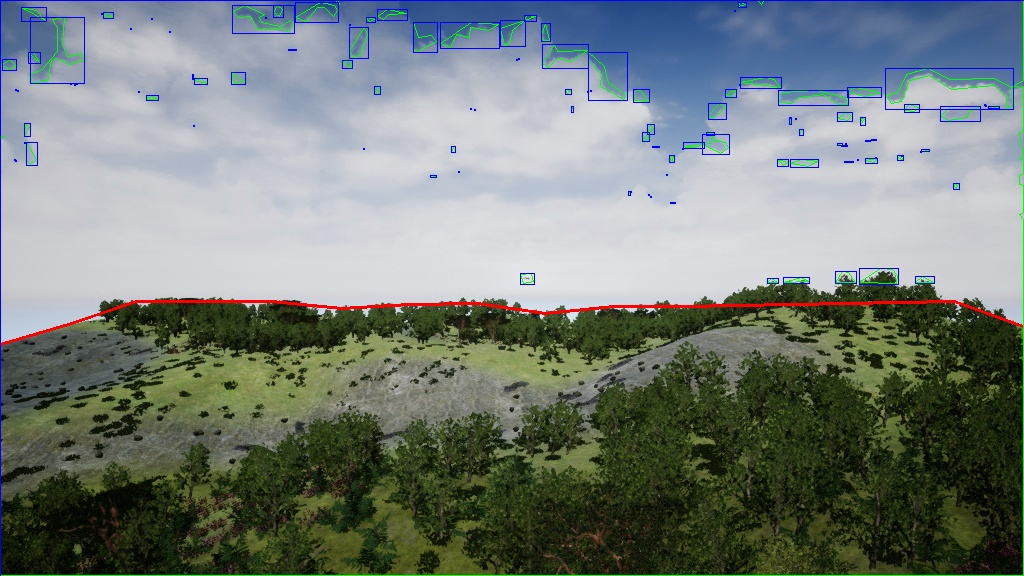
\includegraphics[width=.27\linewidth]{images/airsim_thresh/img_adaptive_3.jpg} &
    % 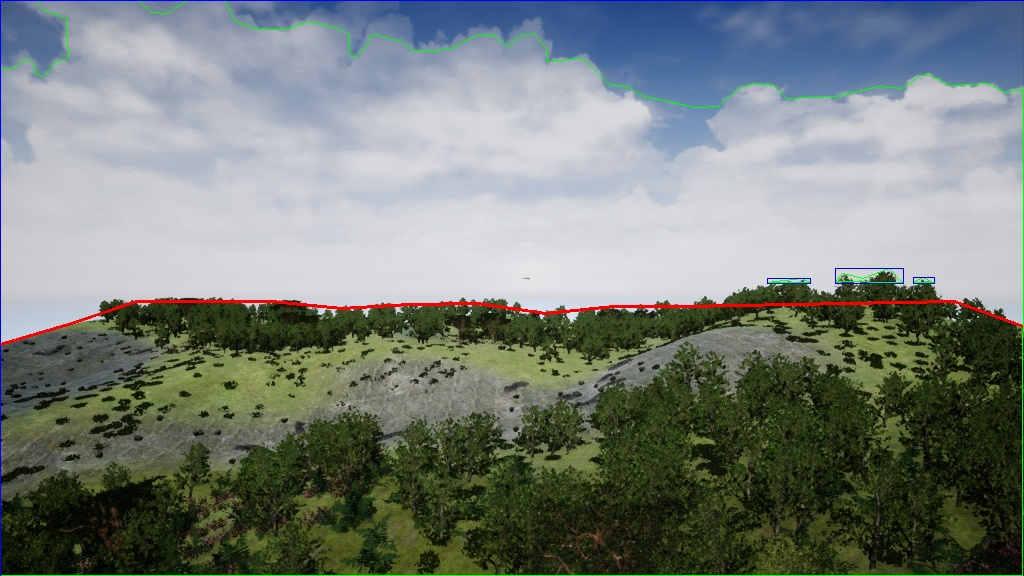
\includegraphics[width=.27\linewidth]{images/airsim_thresh/img_thresh_3.jpg} \\
    
    % 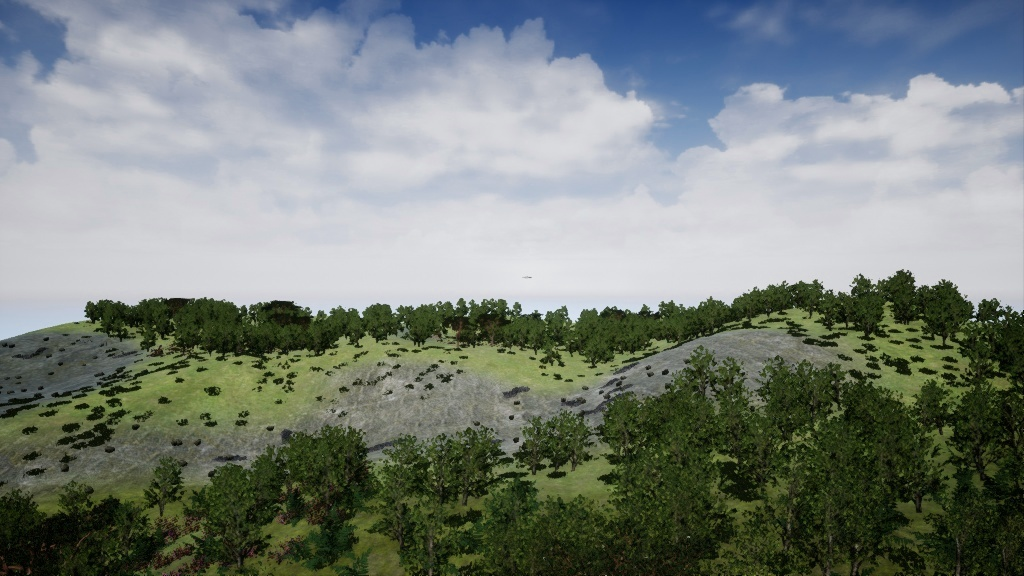
\includegraphics[width=.27\linewidth]{images/airsim_thresh/img_4.jpg} &
    % 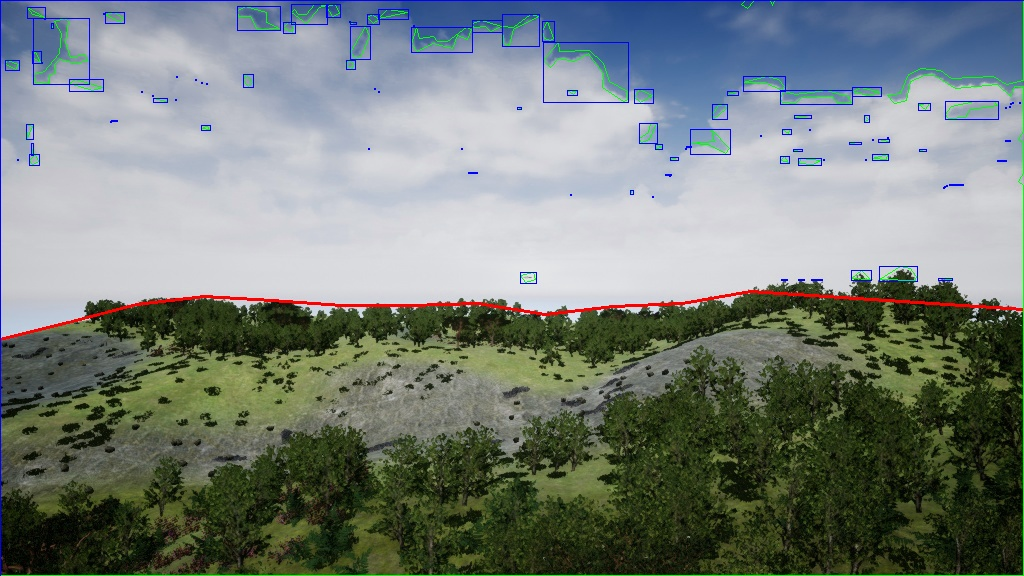
\includegraphics[width=.27\linewidth]{images/airsim_thresh/img_adaptive_4.jpg} &
    % 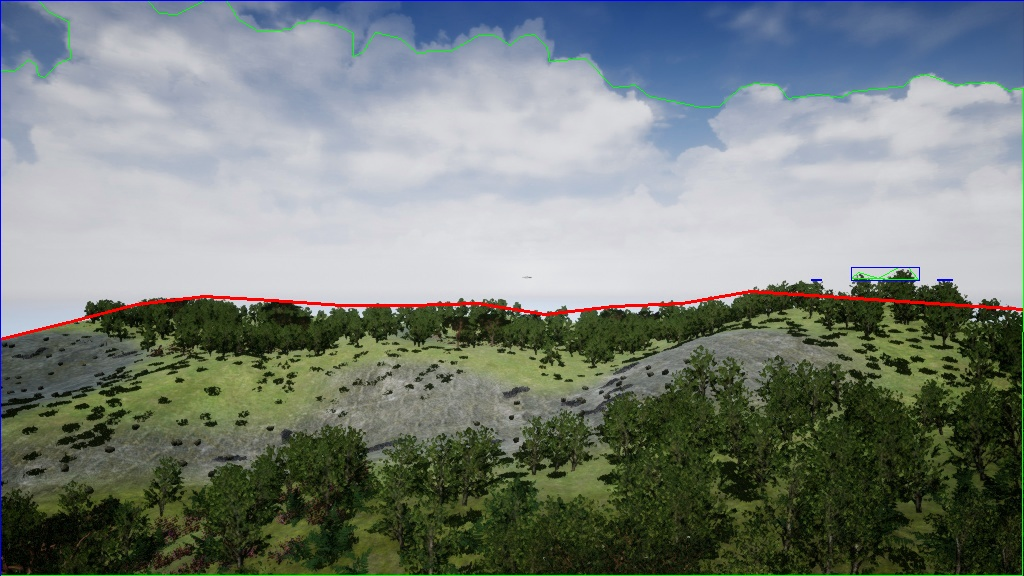
\includegraphics[width=.27\linewidth]{images/airsim_thresh/img_thresh_4.jpg} \\
    
    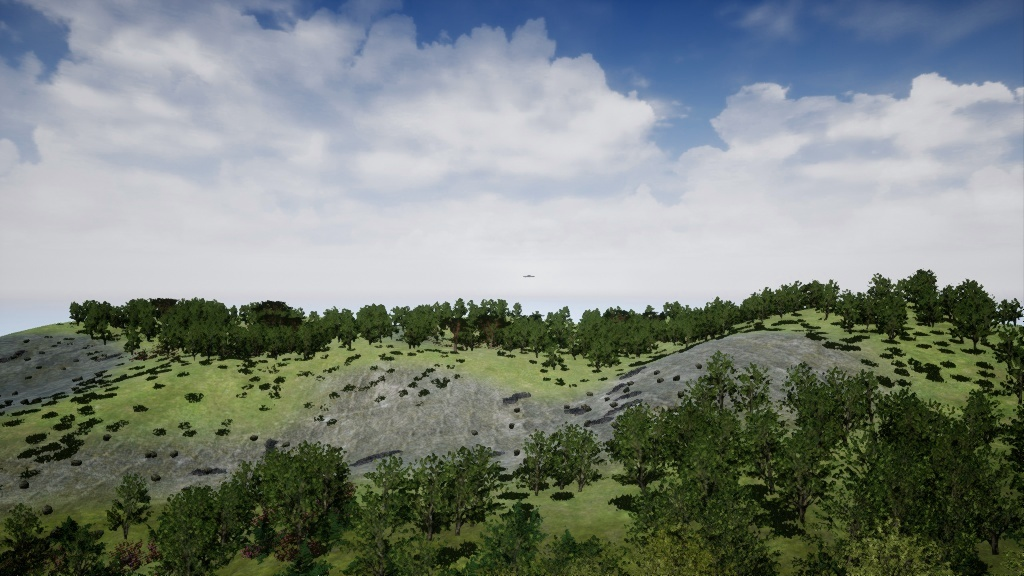
\includegraphics[width=.27\linewidth]{images/airsim_thresh/img_5.jpg} &
    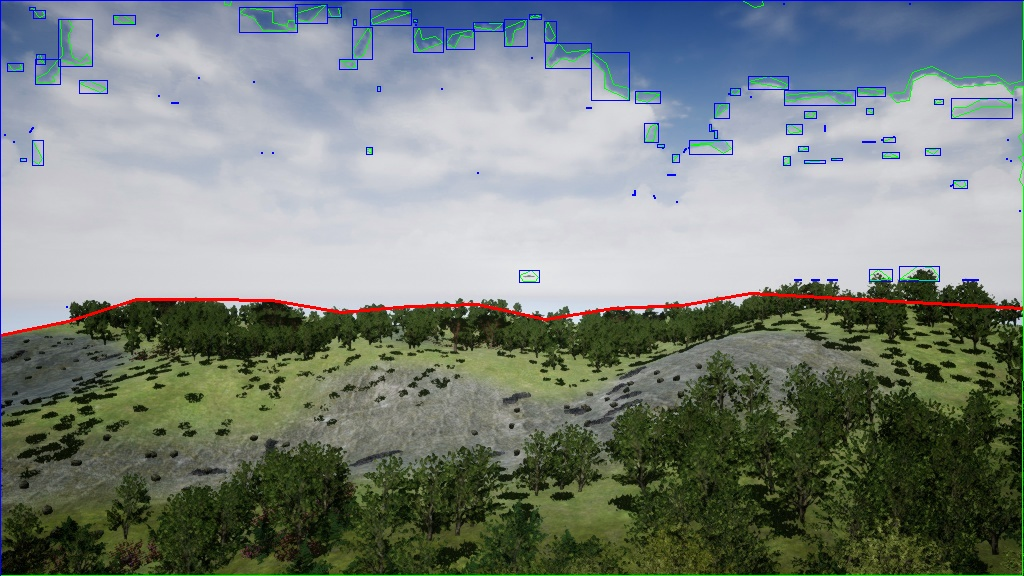
\includegraphics[width=.27\linewidth]{images/airsim_thresh/img_adaptive_5.jpg} &
    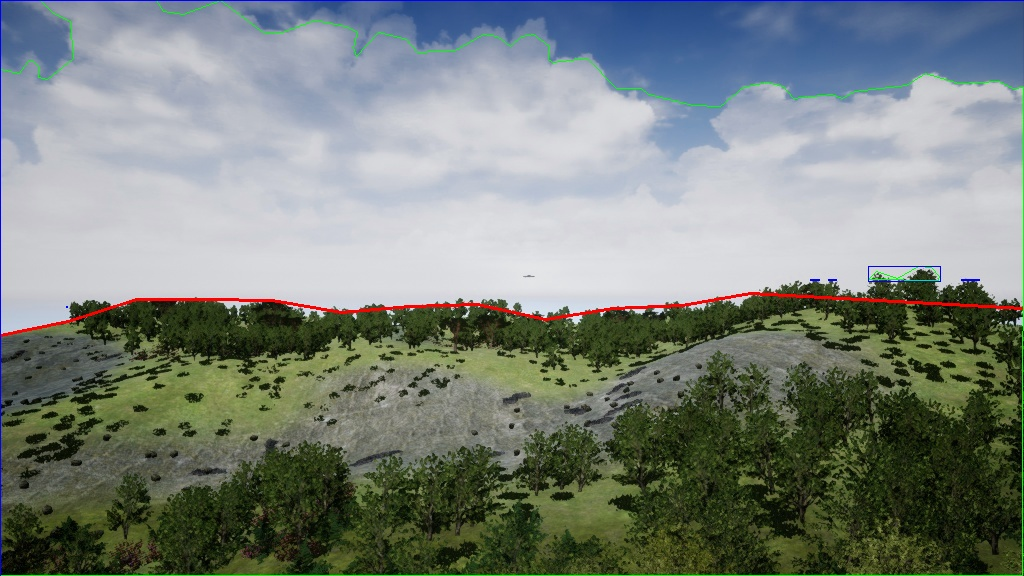
\includegraphics[width=.27\linewidth]{images/airsim_thresh/img_thresh_5.jpg} \\
    
    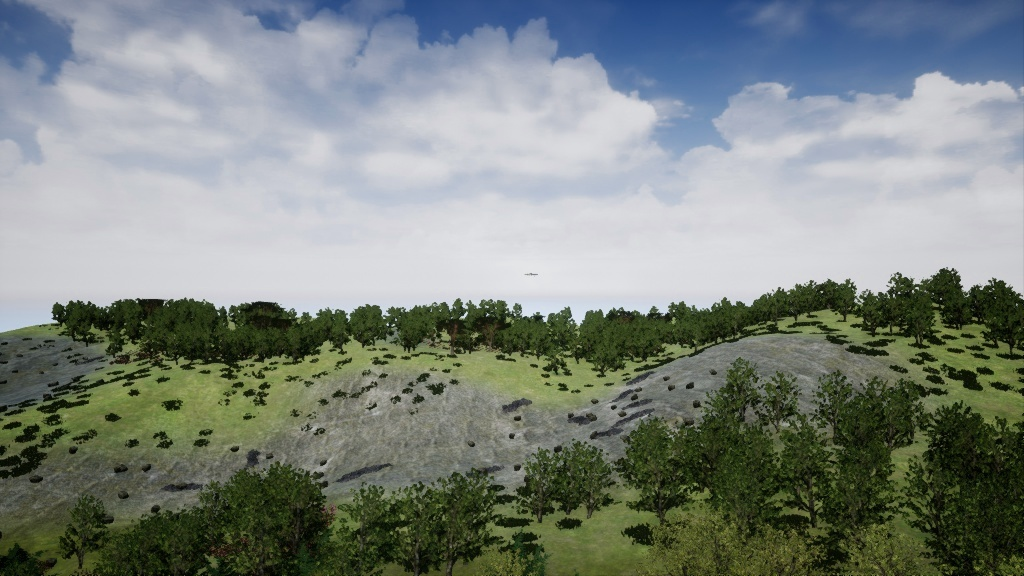
\includegraphics[width=.27\linewidth]{images/airsim_thresh/img_6.jpg} &
    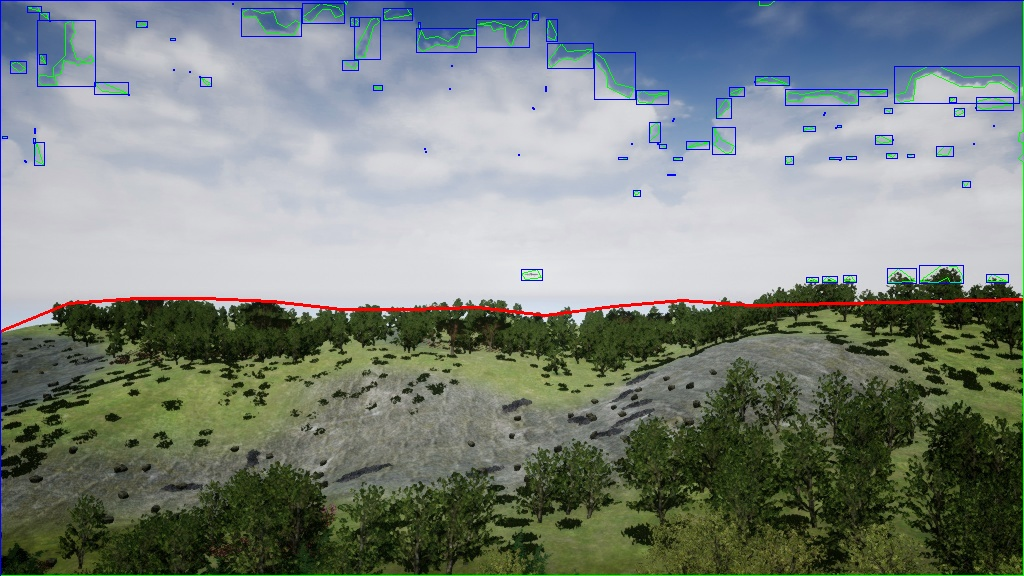
\includegraphics[width=.27\linewidth]{images/airsim_thresh/img_adaptive_6.jpg} &
    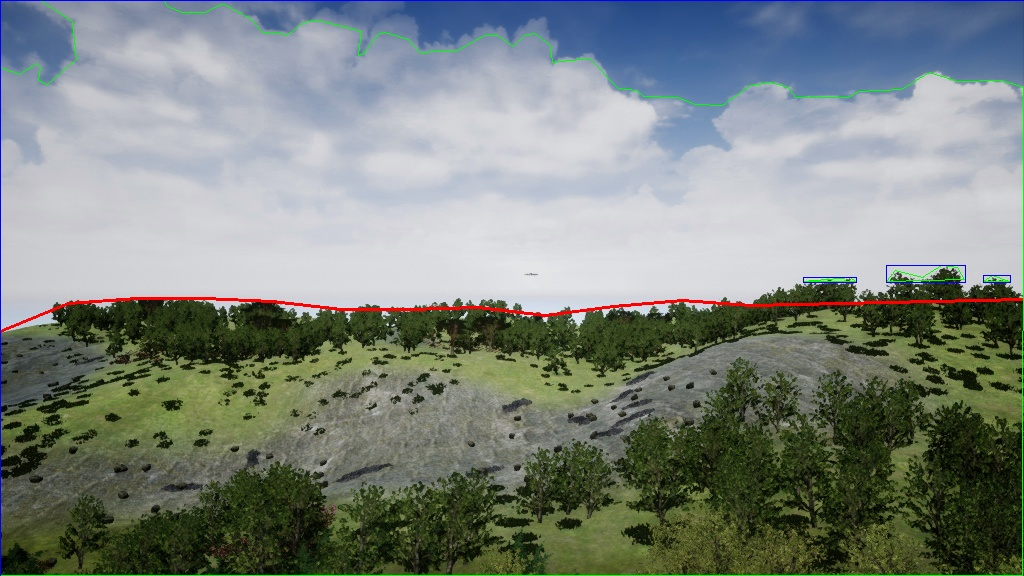
\includegraphics[width=.27\linewidth]{images/airsim_thresh/img_thresh_6.jpg} \\
    
    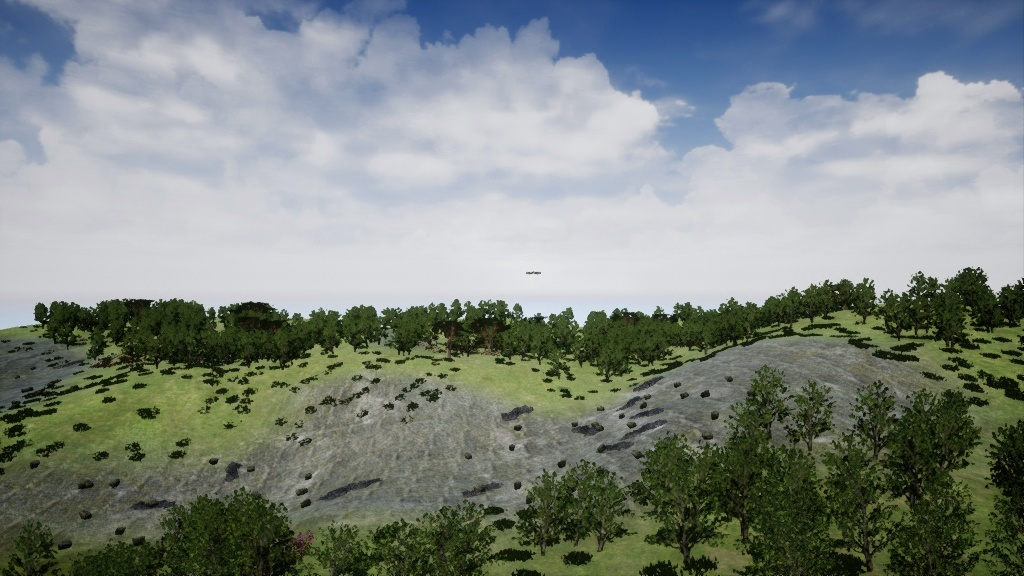
\includegraphics[width=.27\linewidth]{images/airsim_thresh/img_7.jpg} &
    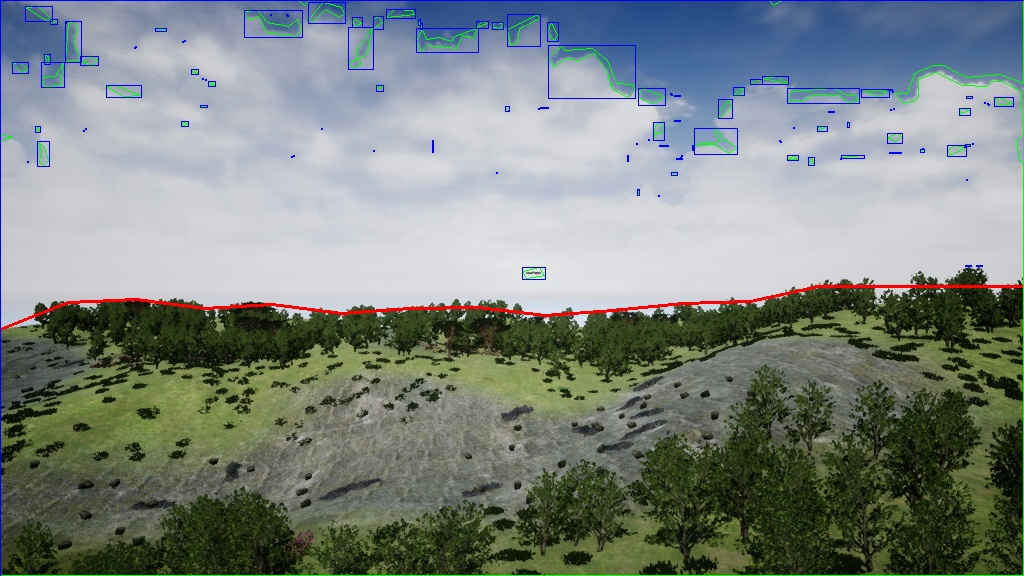
\includegraphics[width=.27\linewidth]{images/airsim_thresh/img_adaptive_7.jpg} &
    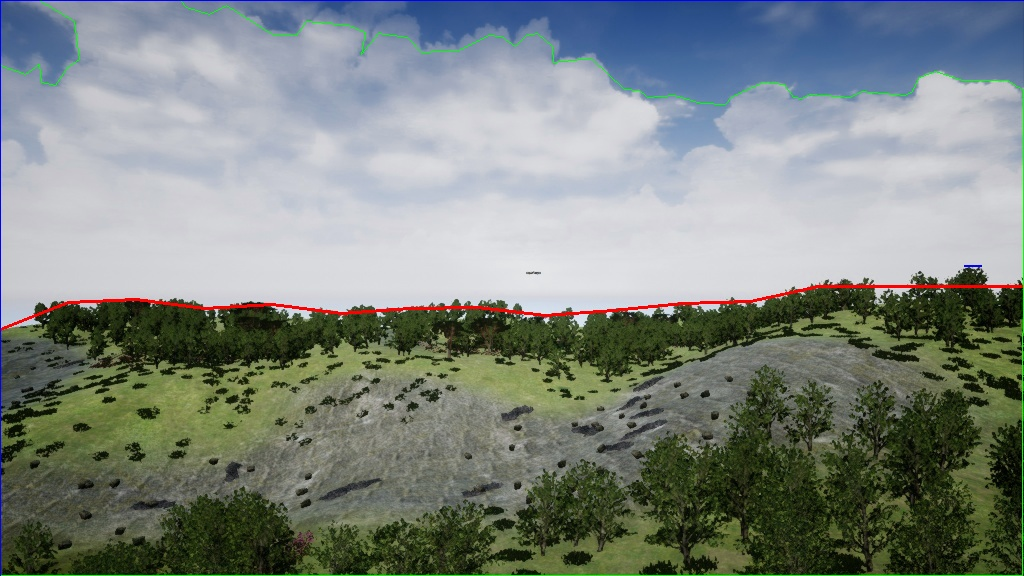
\includegraphics[width=.27\linewidth]{images/airsim_thresh/img_thresh_7.jpg} \\
    
    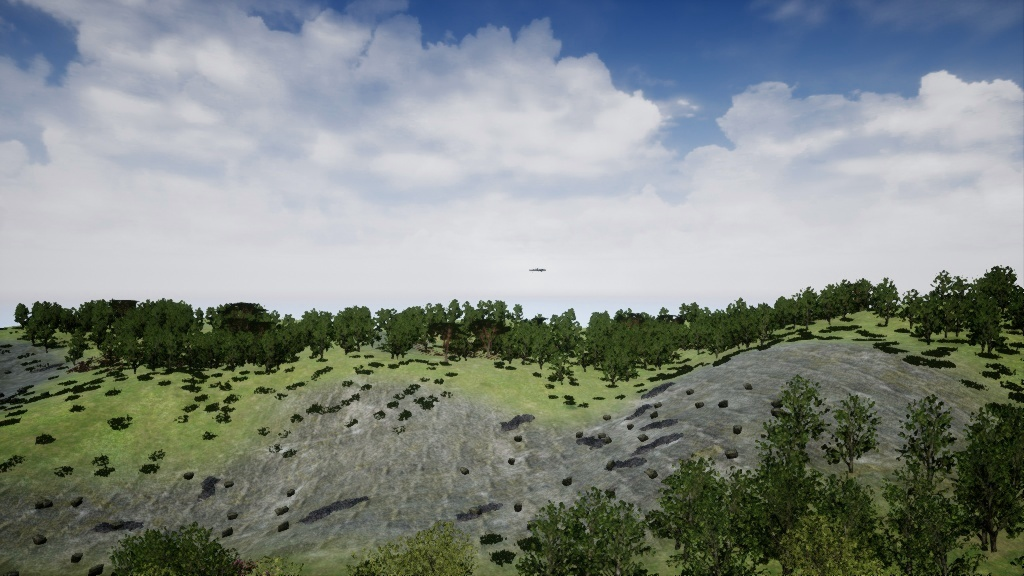
\includegraphics[width=.27\linewidth]{images/airsim_thresh/img_8.jpg} &
    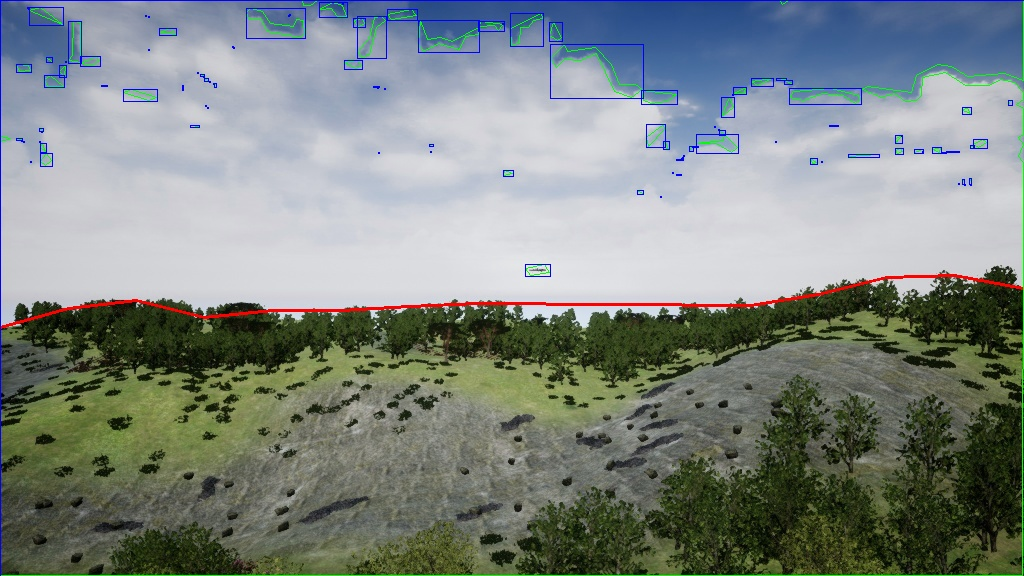
\includegraphics[width=.27\linewidth]{images/airsim_thresh/img_adaptive_8.jpg} &
    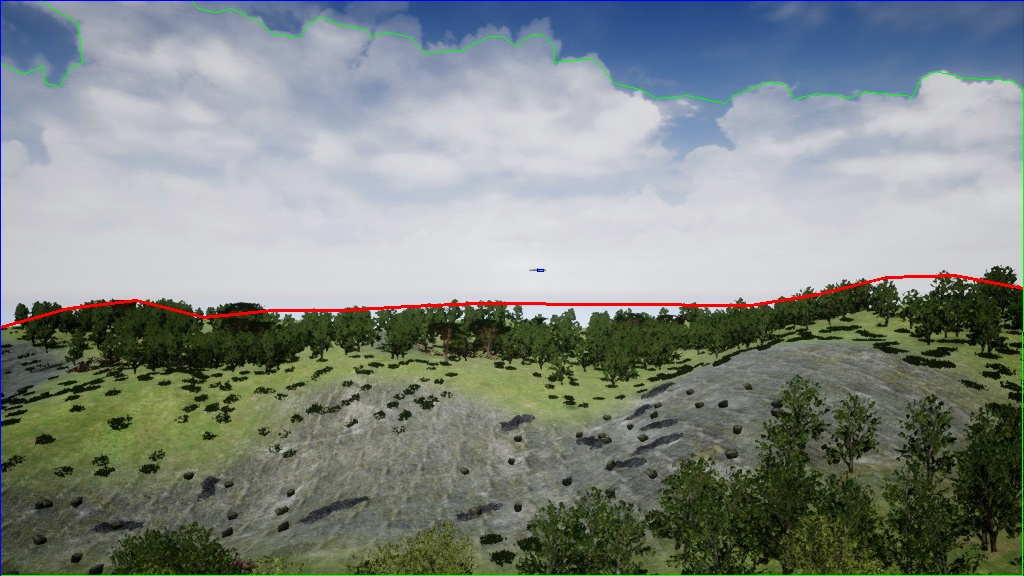
\includegraphics[width=.27\linewidth]{images/airsim_thresh/img_thresh_8.jpg} \\
    
    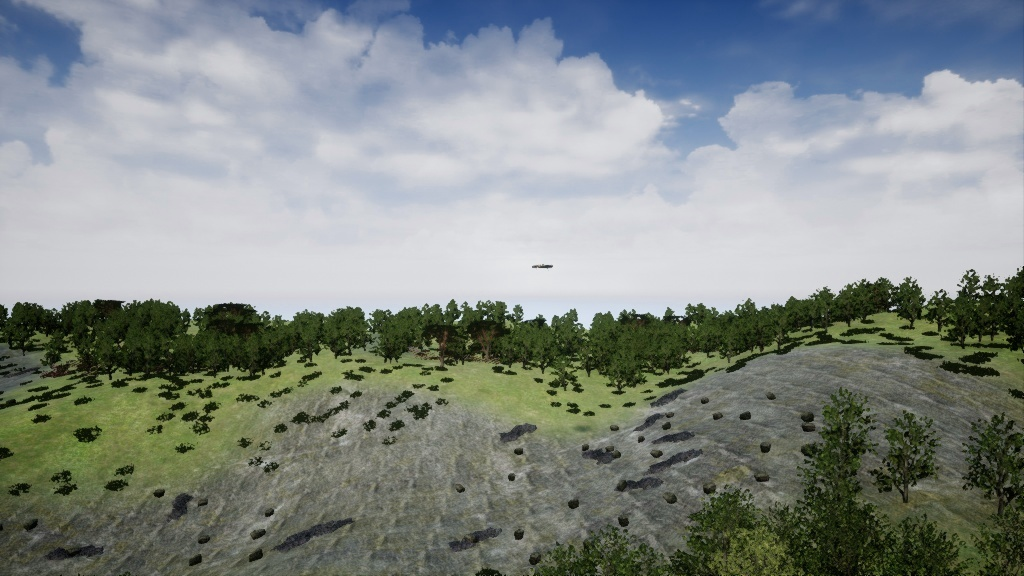
\includegraphics[width=.27\linewidth]{images/airsim_thresh/img_9.jpg} &
    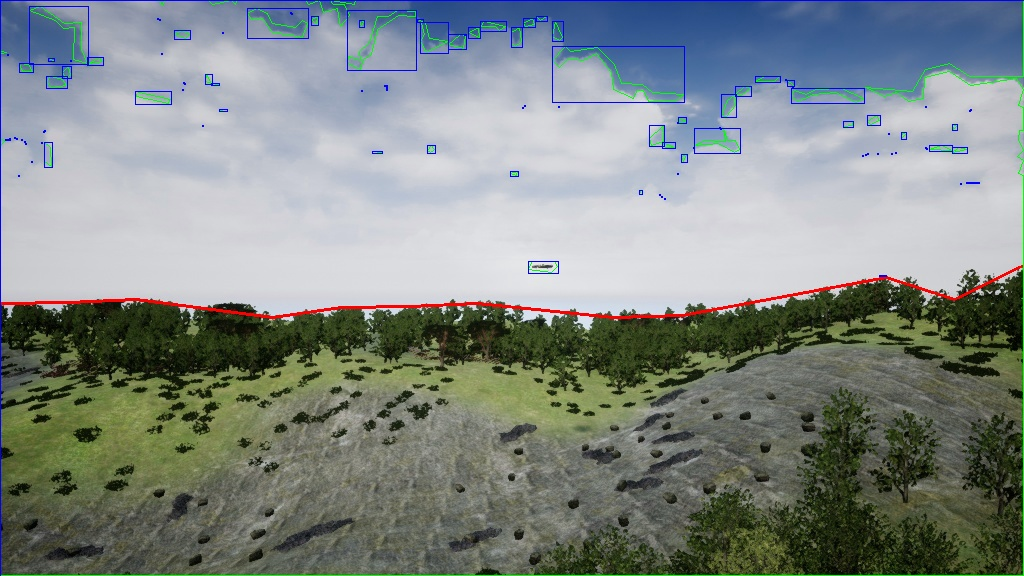
\includegraphics[width=.27\linewidth]{images/airsim_thresh/img_adaptive_9.jpg} &
    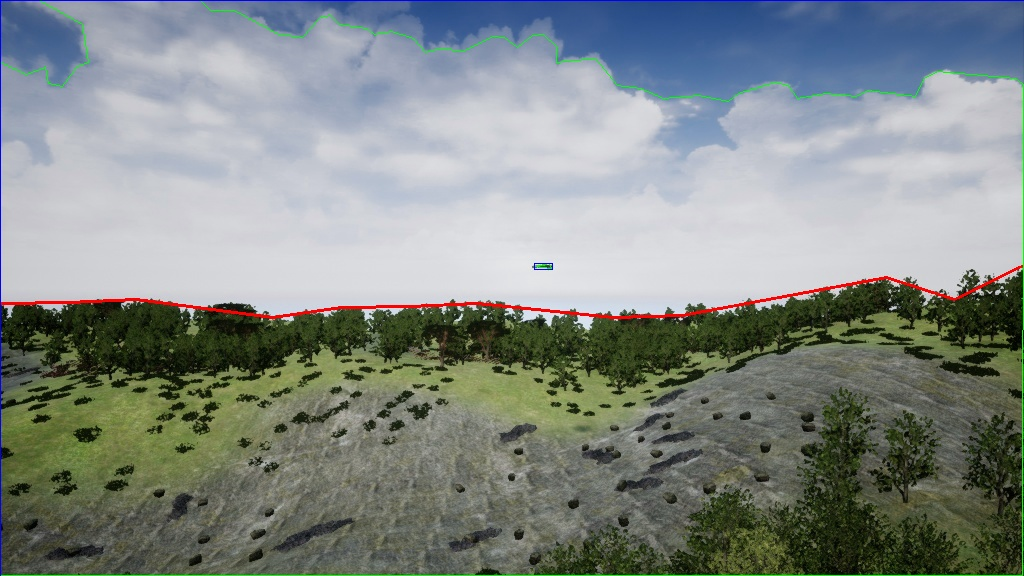
\includegraphics[width=.27\linewidth]{images/airsim_thresh/img_thresh_9.jpg} \\
    
    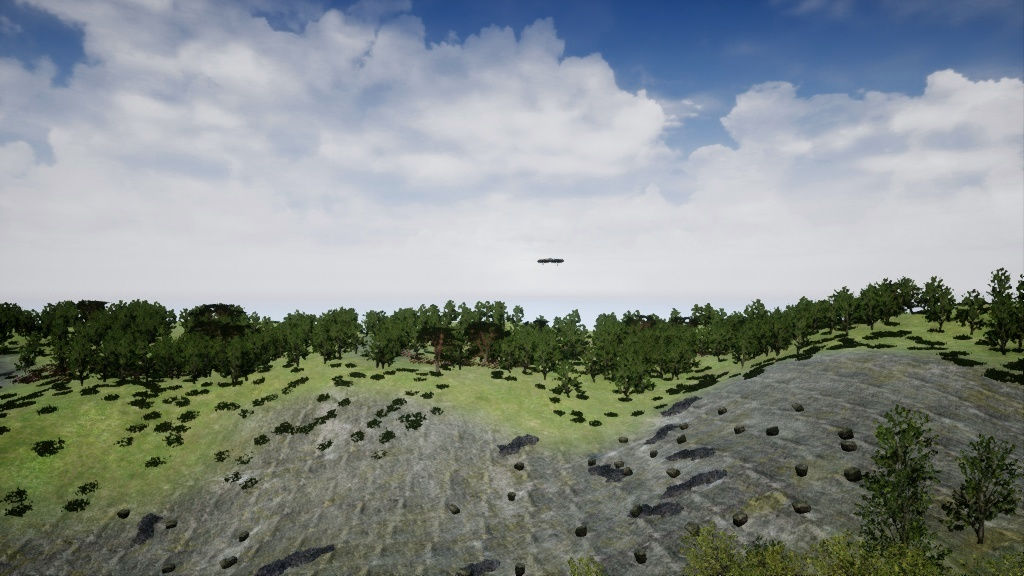
\includegraphics[width=.27\linewidth]{images/airsim_thresh/img_10.jpg} &
    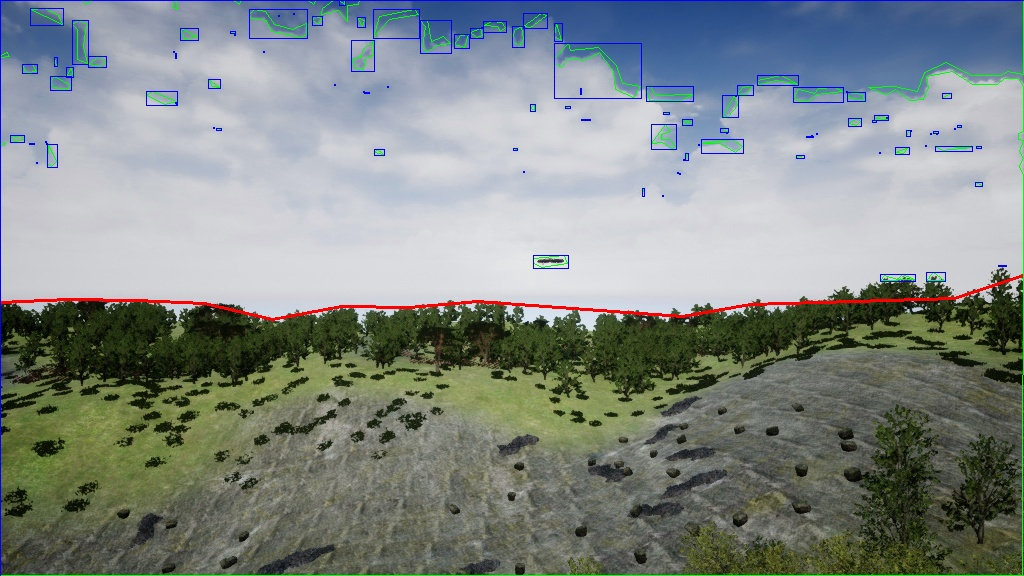
\includegraphics[width=.27\linewidth]{images/airsim_thresh/img_adaptive_10.jpg} &
    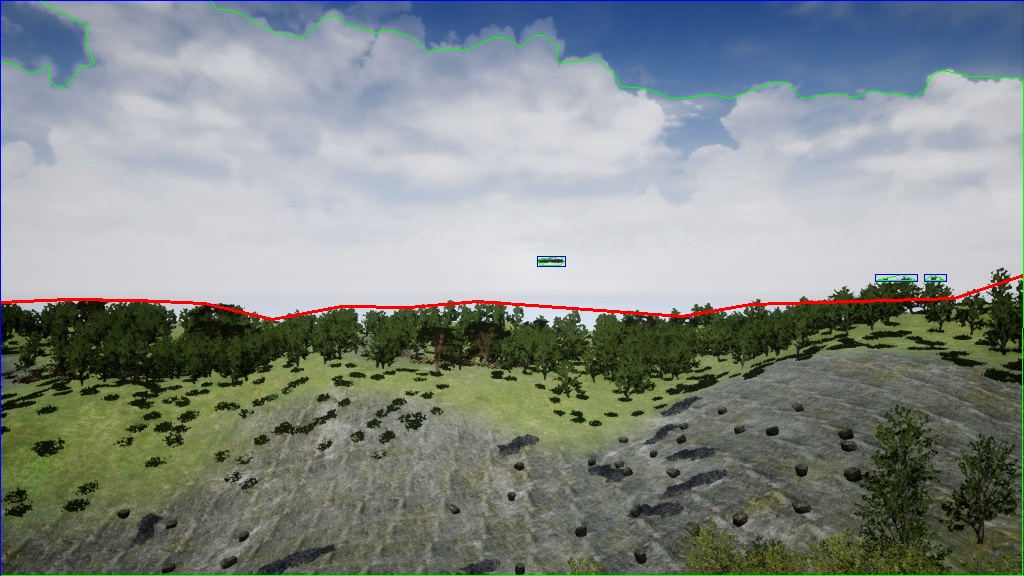
\includegraphics[width=.27\linewidth]{images/airsim_thresh/img_thresh_10.jpg} \\
    
    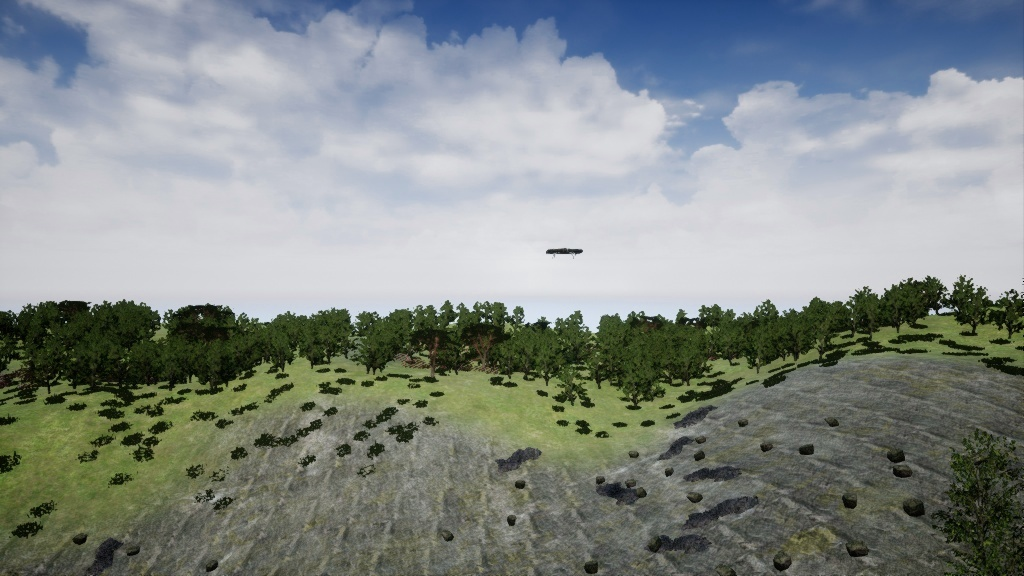
\includegraphics[width=.27\linewidth]{images/airsim_thresh/img_11.jpg} &
    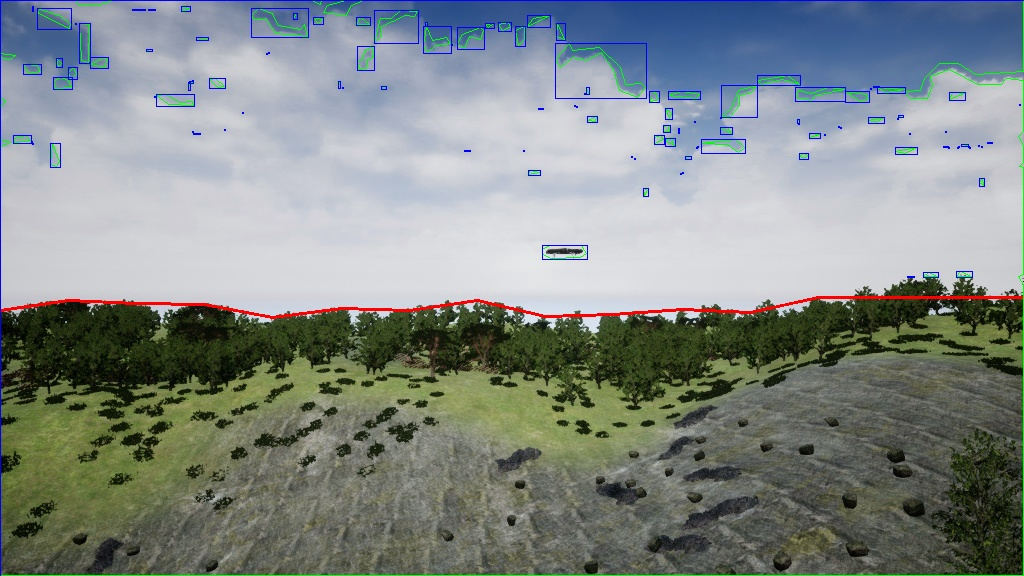
\includegraphics[width=.27\linewidth]{images/airsim_thresh/img_adaptive_11.jpg} &
    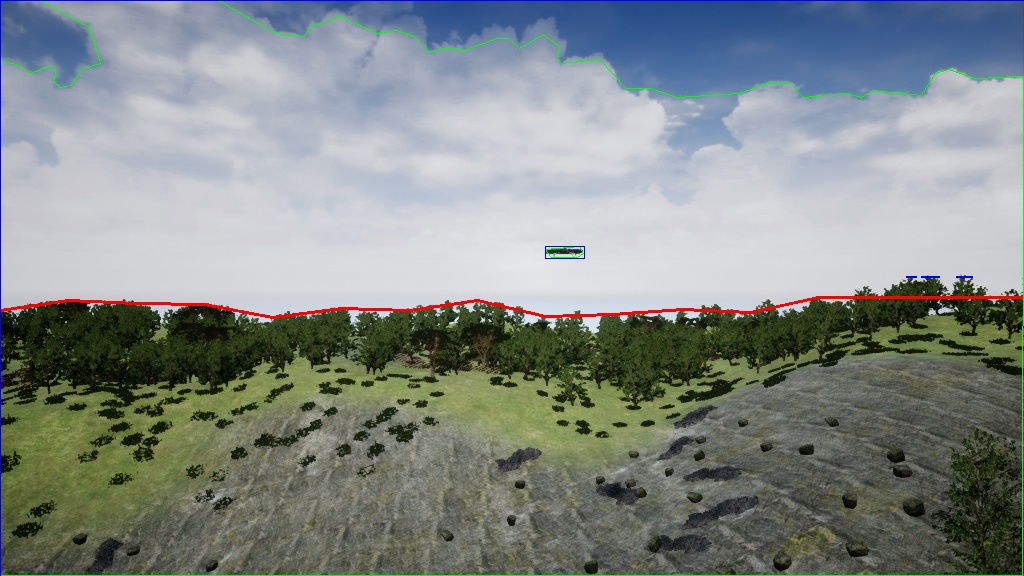
\includegraphics[width=.27\linewidth]{images/airsim_thresh/img_thresh_11.jpg} \\
    
    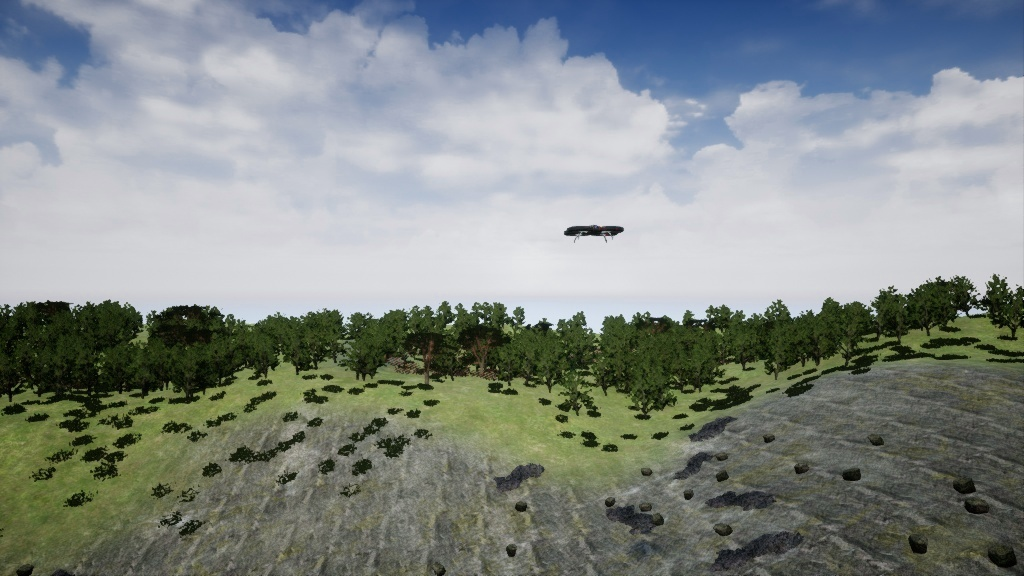
\includegraphics[width=.27\linewidth]{images/airsim_thresh/img_12.jpg} &
    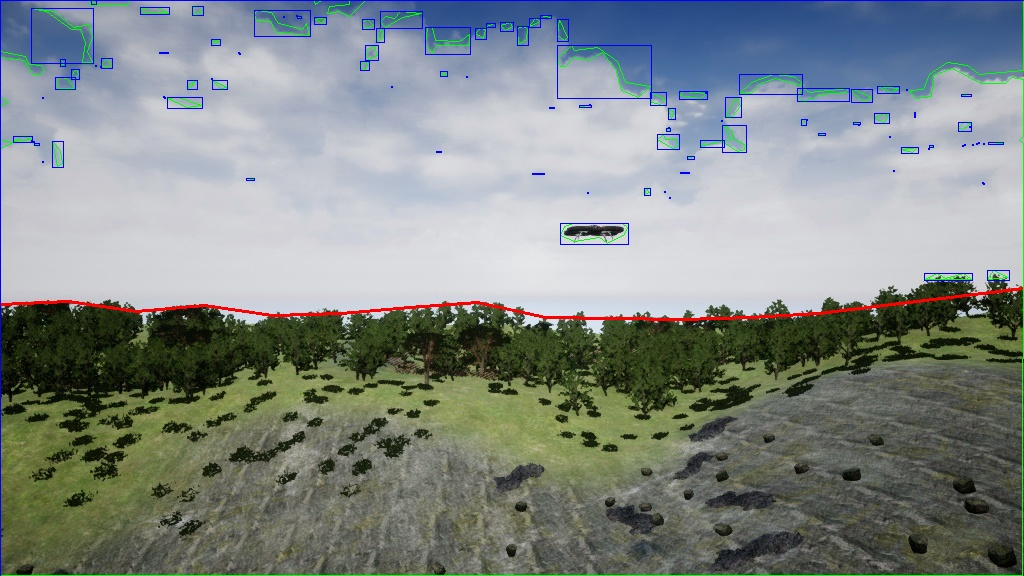
\includegraphics[width=.27\linewidth]{images/airsim_thresh/img_adaptive_12.jpg} &
    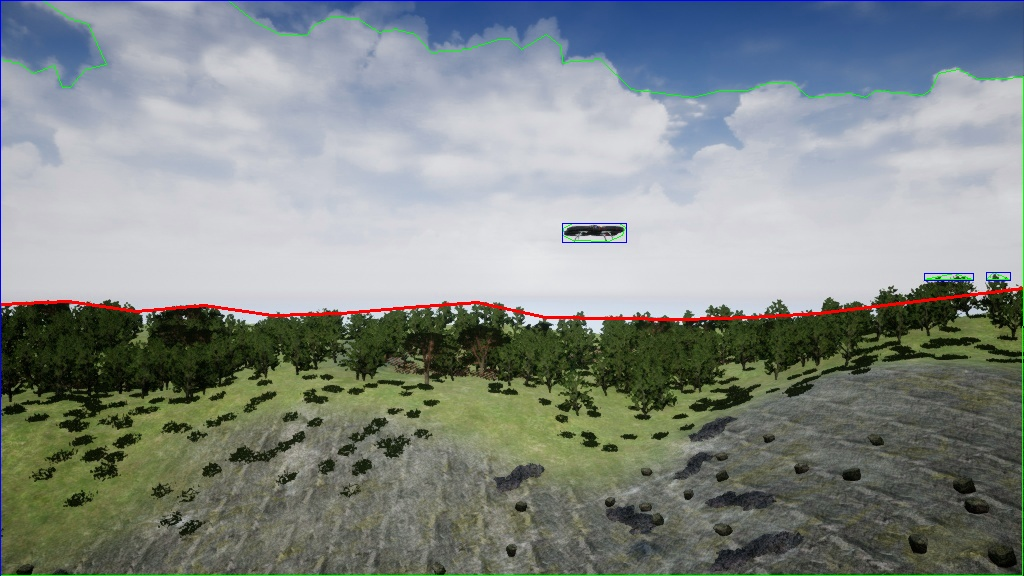
\includegraphics[width=.27\linewidth]{images/airsim_thresh/img_thresh_12.jpg} \\
    
    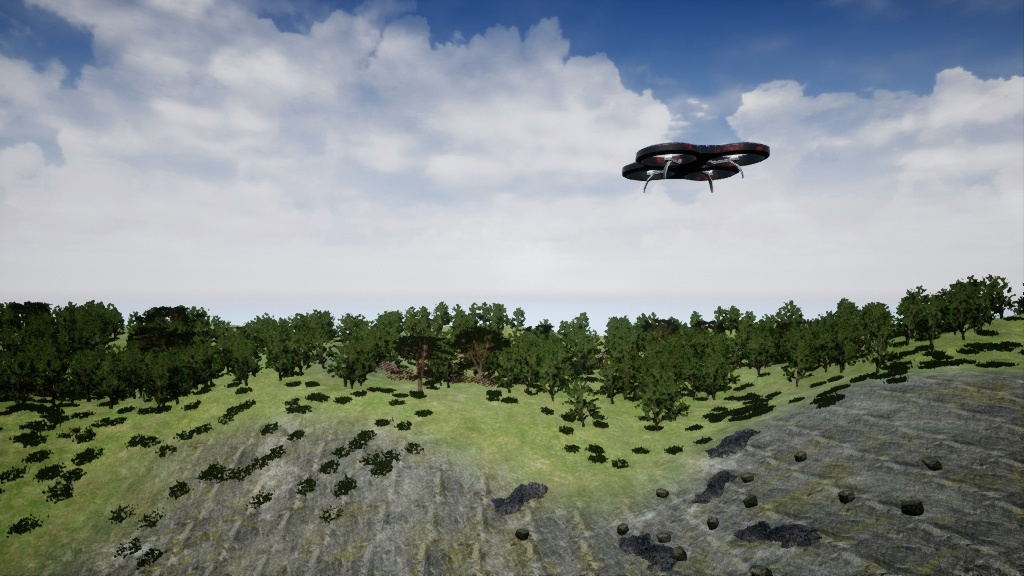
\includegraphics[width=.27\linewidth]{images/airsim_thresh/img_13.jpg} &
    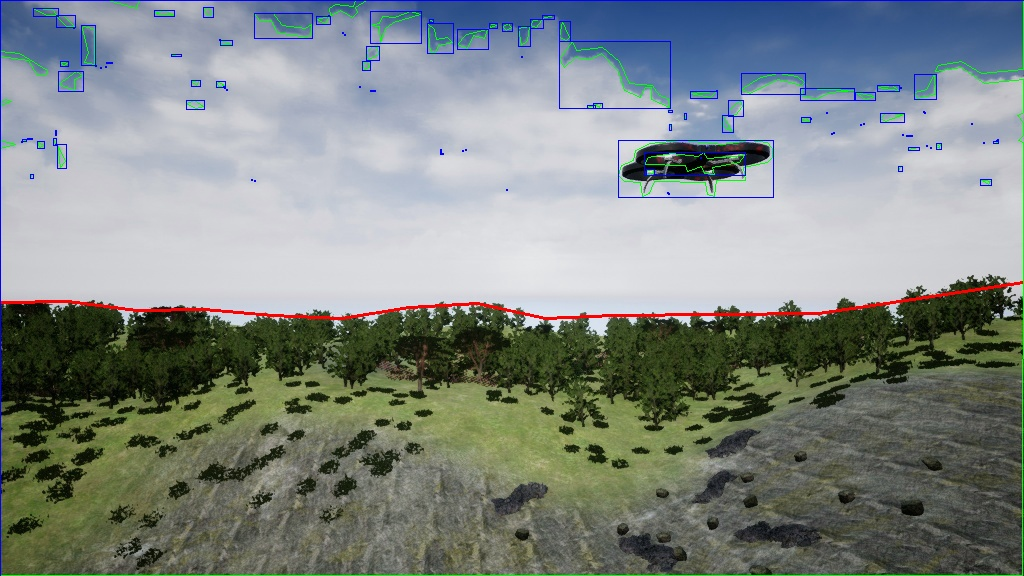
\includegraphics[width=.27\linewidth]{images/airsim_thresh/img_adaptive_13.jpg} &
    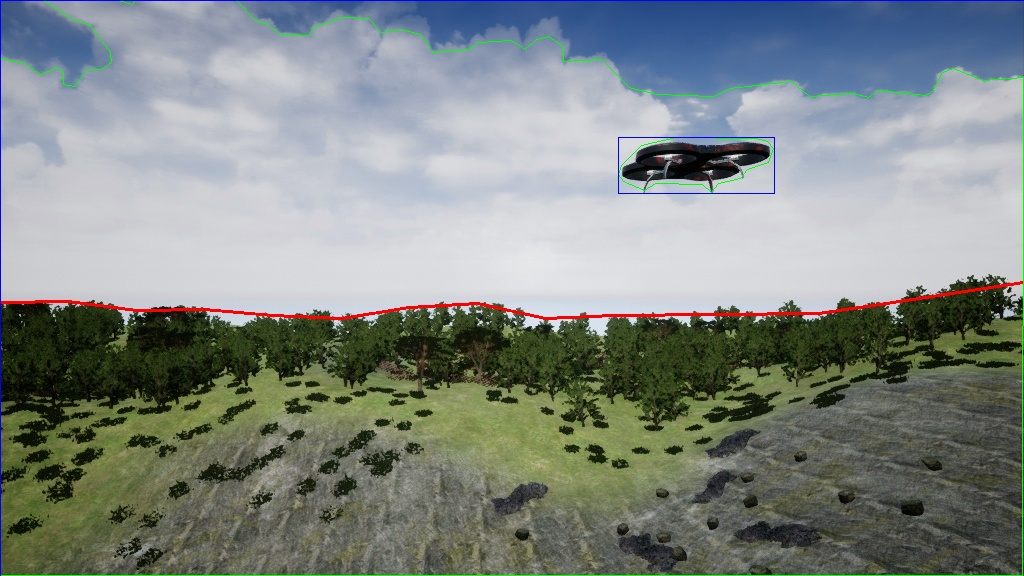
\includegraphics[width=.27\linewidth]{images/airsim_thresh/img_thresh_13.jpg} \\
    \end{tabular}
    \caption{Comparition of threshold and adaptive-threshold}
    \label{fig:thresh_compar}
\end{figure}
\clearpage

\section{HLS Prepocess} % 3401 characters

The implemented solution of the preprocessing block is the same as in the python block.
In C however, there must be temporary storage to be specified (line 17,21,23,29)
These variables later will be optimised according to the directives.
There can be seen temporarily removed lines that are corresponding with the Otsu threshold, and the adaptive threshold implementations.
The Otsu method was removed due to dataflow optimizations, but the threshold value is set according to offline Otsu calculations.
The adaptive threshold had too much error, hence it ruined the otherwise proper algorithm.
The other interesting part of this code is the streaming interface, and the xf::Mat conversation.
To transfer data to the FPGA, an AXI interface must be used.
The synthesis is not able to convert a struct or class to AXI data, thus other means of data transfer should be implemented.
The easiest is to transfer an array of data, which is a convenient solution, however, due to type conversations (change between OpenCV pixel type, AXI type, and xcOpenCV type) this solution was not feasible.
The other solution which requires more work and programming is to transfer the data through a stream.
For this, the VDMA is required.
The HLS generated IP has to be connected to the ZYNQ subsystem and the VDMA in and out streaming ports.
The system after uploading the preprocess block with the required kernels (all kernels require a separate kernel port to keep the dataflow) and sizes, the VDMA can be started as well.
The memory addresses should be set, for the python program to save the image to the read address offset of the VDMA.
The VDMA than creates a stream of the memory and transfers the data to the preprocessing.
The output of the preprocess sends the data back to the VDMA, that saves that data to a separate place on the memory.
the python system can read the memory and continue, with the processed image.
The uploading of the boxes can be done before the system start but the image load and write must be waited for.
This plus the latency of the system can cause async execution of the code.
This has to be handled by the python program as well.

\begin{figure}
    \centering
    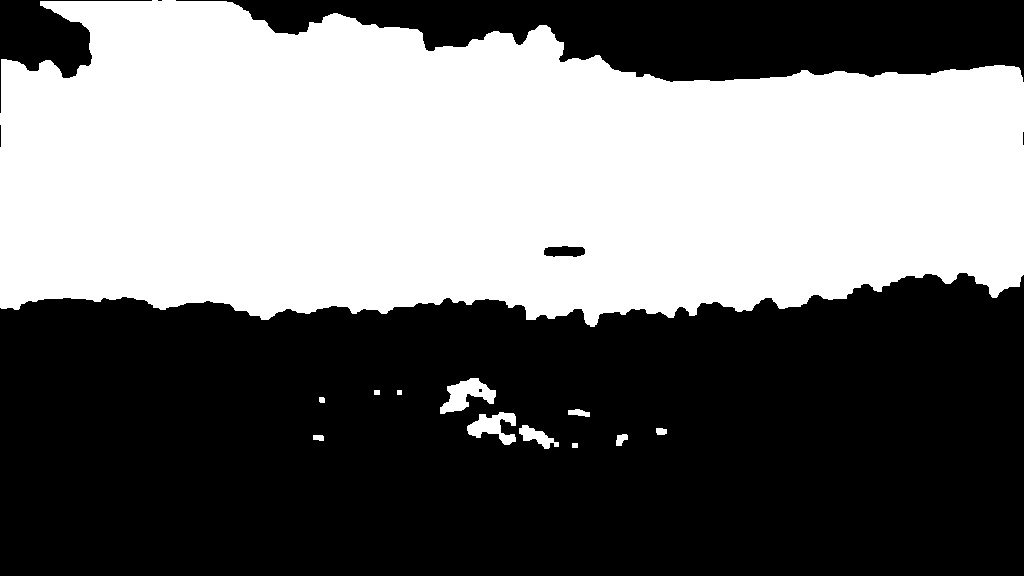
\includegraphics[width=.32\linewidth]{images/preproc/out_ocv.jpg}
    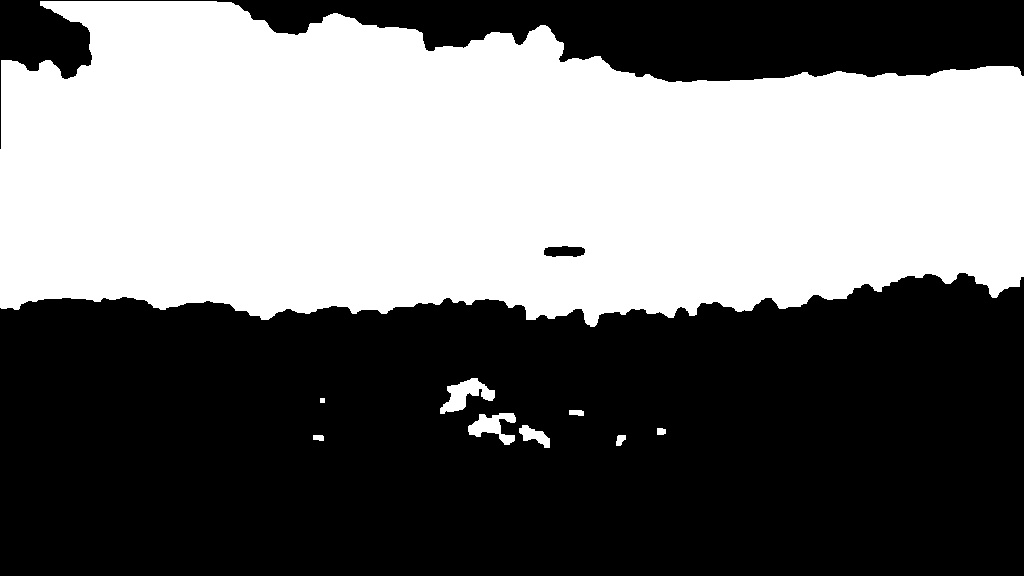
\includegraphics[width=.32\linewidth]{images/preproc/hls_out.jpg}
    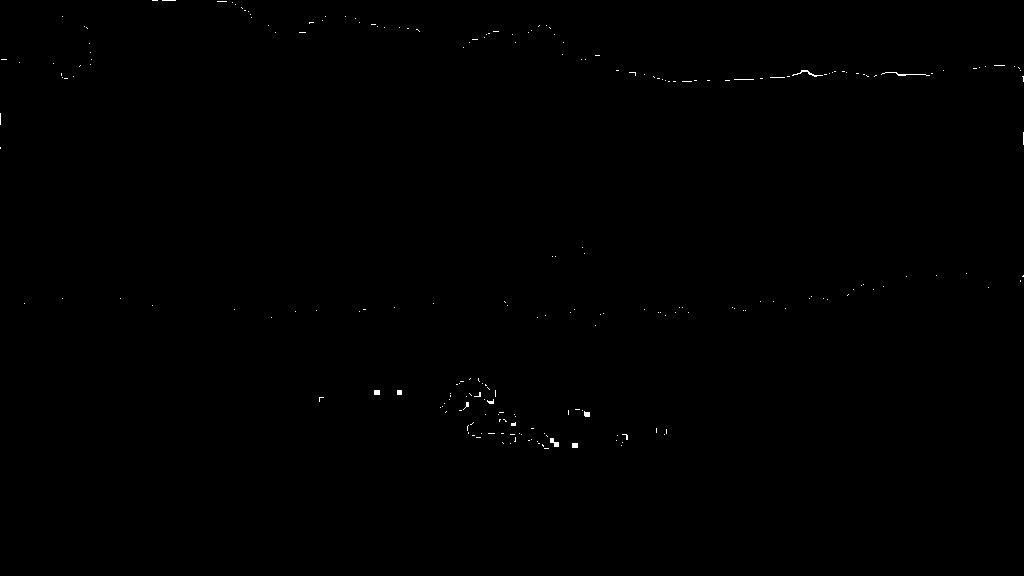
\includegraphics[width=.32\linewidth]{images/preproc/error.png}
    \caption{Preprocessing comparation of the OpenCV image, the HLS block, and the visual differences.}
    \label{fig:preproc_compare}
\end{figure}

To validate the software, a test bench source (\cref{code:test_bench}) was made.
This source is also required by the Synthesis and the simulation processes of the HLS.
In this program, the same image is processed by both the original OpenCV and the HLS block as well.
The HLS block is a simulated process, which means that the computer tries to replicate the effect of the directives in an SI processor.
This requires a lot of time, and resource, and also in some cases (eg. loading in a FIFO) not even possible to implement.
The HLS tries to calculate the parameters of the hardware and compares it to the results of the simulated run.
If the values are correct the original and the hardware implementation results are compared (line 36-56).
To have a reference to compare, a series of OpenCV function was introduced to the test bench (line 13-18).
These functions are the C implementations instead of the python, which is used in the algorithm, but the underlying logic is the same.
The OpenCV installed on the computer is also compiled in release more, hence the functionalities are all optimised.
After the reference image, the data is converted to a hls::stream (line 24), for easier transfer.
The stream is fed to the block and the output stream is written back to another image (line 28).
After the results are written in two variable, by both the OpenCV and the HLS block as well, the difference between the two is calculated (line 32).
The test showed an average of 0.150892\%of pixels above the error threshold.
Here a simple differential calculation is used, but in some cases, other error measures had to be introduced.
All three image is written to the disc for visual comparison (line 20,30,34) (\cref{fig:preproc_compare}).

The final system and the HLS implementation results can be seen in \cref{tab:preproc_hls_usage}.
The minimal and the maximal latency is between 8321540 and 8331485, where the greatest contributor is the Gaussian Blur and the Threshold (\cref{tab:preproc_hls_latency}).
After adding the connectivity and the VDMA to the design file, the system utilization got a little higher (\cref{tab:preproc_final_usage}).

\begin{table}
    \centering
    \caption{Preprocessing HLS block hardware requirements}
    \label{tab:preproc_hls_usage}
    \begin{tabular}{|l|l|l|l|l|l|}
    \hline
    Name &  BRAM\_18K &  DSP48E &  FF &  LUT &  URAM \\ \hline
    DSP & - & - & - & - & - \\ \hline
    Expression & - & - & 0 & 71 & - \\ \hline
    FIFO & 0 & - & 171 & 1316 & - \\ \hline
    Instance & 46 & 4 & 7617 & 13636 & - \\ \hline
    Memory & - & - & - & - & - \\ \hline
    Multiplexer & - & - & - & 90 & - \\ \hline
    Register & - & - & 15 & - & - \\ \hline
    Total & 46 & 4 & 7803 & 15113 & 0 \\ \hline
    Available & 1824 & 2520 & 548160 & 274080 & 0 \\ \hline
    Utilization (\%) & 2 & $\approx$ 0 & 1 & 5 & 0 \\ \hline
    \end{tabular}
\end{table}

\begin{table}
    \centering
    \caption{Latency measurements of the main components on the Preprocess block}
    \label{tab:preproc_hls_latency}
    \begin{tabular}{|l|c|c|c|c|}
    \hline
    Module & Latency & & Interval \\ \hline
    & min &  max &  min &  max \\ \hline
    erode90 & 105 & 8331455 & 105 & 8331455 \\ \hline
    erode & 105 & 8331455 & 105 & 8331455 \\ \hline
    dilate & 105 & 8331455 & 105 & 8331455 \\ \hline
    GaussianBlur & 8321526 & 8321526 & 8321526 & 8321526  \\ \hline
    xfMat2AXIvideo & 1 & 8303041 & 1 & 8303041 \\ \hline
    AXIvideo2xfMat & 3 & 8305203 & 3 & 8305203 \\ \hline
    Threshold & 8300881 & 8300881 & 8300881 & 8300881 \\ \hline
    \end{tabular}
\end{table}

% \begin{table}
% \centering
% \caption{Clocking results for the Preprocess block}
% \label{tab:preproc_hls_timing}
% \begin{tabular}{|l|l|}
% \hline
% \end{tabular}
% \end{table}

\begin{table}
\centering
\caption{Final preprocess Overlay utilization table}
\label{tab:preproc_final_usage}
\begin{tabular}{|l|l|l|l|}
\hline
Resource & Utilization & Available & Utilization \% \\ \hline
LUT & 15725 & 274080 & 5.74 \\ \hline
LUTRAM & 2674 & 144000 & 1.86 \\ \hline
FF & 20511 & 548160 & 3.74 \\ \hline
BRAM & 34 & 912 & 3.73 \\ \hline
DSP & 4 & 2520 & 0.16 \\ \hline
BUFG & 1 & 404 & 0.25 \\ \hline
\end{tabular}
\end{table}

%!!! POWER REPORT KELL IDE IS

\clearpage

\section{Adaptive Threshold} % 1670 characters
The adaptive threshold function is one of the used OpenCV function of the avoid algorithm.
This function, however, is not implemented in the xhOpenCV library, hence it has been replicated according to the OpenCV implementation.
For this, another HLS block was created (\cref{code:adaptive_thrash}).
The first approach was to modify the custom convolution implementation of the xfOpenCV.
This required to remove the kernel input of the function and add a division at the end of the kernel function.
The resulting algorithm did not satisfy the correctness criteria of error measure beeing under 1\%.
The function also required to use of a modified function of an already validated one.
This makes the further development hard, and the maintenance of the current code a nightmare.
After studying the code of the original OpenCV implementation, the obvious solution became clear.
In the Original library, the Adaptive threshold is not implemented with a dedicated function, but a box filter chained with a decision logic.
By chaining this two logic the end result seemed to be satisfied until the function was not connected to other functions.
As it turns out the error measure at the validation of the boxFilter solution in the xfOpenCV library is not set up for matching the original exactly but allows the values to jitter by 1 (\cref{code:box_error}).
At first, it can not be seen on the image, but when multiple functions are applied to the output of the boxFilters this error can result in a huge difference.

\lstset{
    language=C,
    caption={Error measure of the Boxfilter algoritm in the xfOpenCV library},
    label={code:box_error},
    keywordstyle=\color{red},
    stringstyle=\color{blue},
    commentstyle=\color{green},
    morecomment=[l][\color{magenta}]{\#},
    columns=fullflexible,
    breaklines=true,
    postbreak=\mbox{\textcolor{red}{$\hookrightarrow$}\space},
}
\begin{lstlisting}
double minval=256,maxval=0;
	int cnt = 0;
	for (int i=0;i<in_img.rows;i++)
	{
		for(int j=0;j<in_img.cols;j++)
		{
			uchar v = diff.at<uchar>(i,j);
			if (v>1)
				cnt++;
			if (minval > v )
				minval = v;
			if (maxval < v)
				maxval = v;
		}
	}
	float err_per = 100.0*(float)cnt/(in_img.rows*in_img.cols);
\end{lstlisting}

\begin{figure}[b]
    \centering
    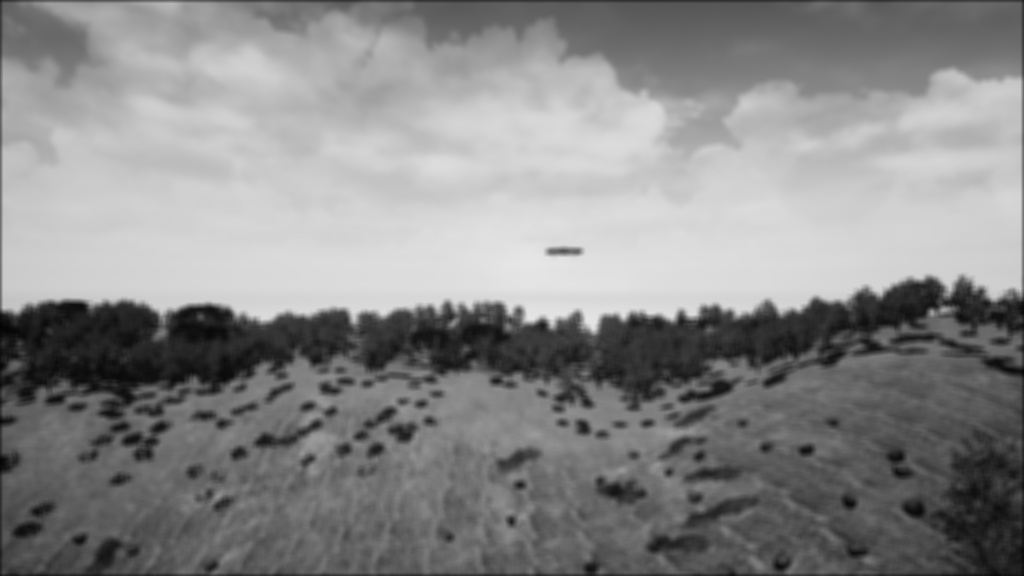
\includegraphics[width=.32\linewidth]{images/box_filter/HLS_img.jpg}
    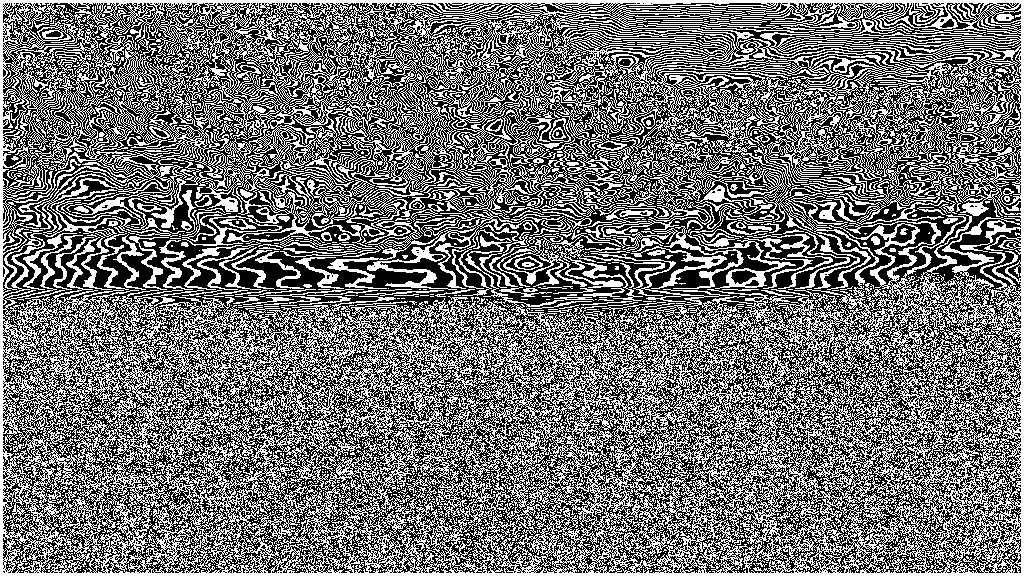
\includegraphics[width=.32\linewidth]{images/box_filter/diff_img.jpg}
    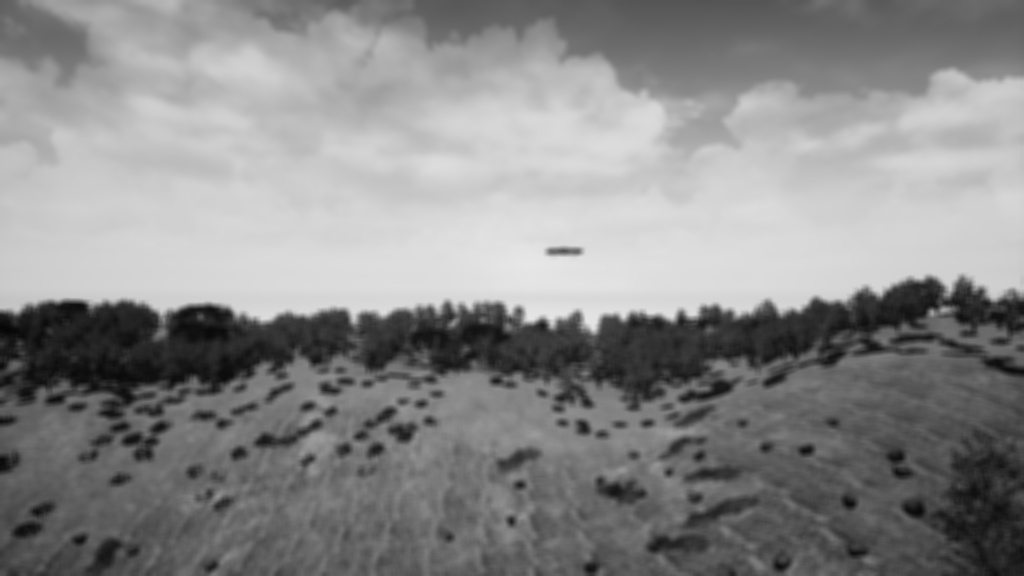
\includegraphics[width=.32\linewidth]{images/box_filter/OCV_img.jpg}
    \caption{The xfOpenCV boxFilter, the difference and the OpenCV boxFilter final result. The error is enhancet for better visual comparation}
    \label{fig:box_error}
\end{figure}

After correcting the error measure, the difference is still hardly noticeable, since it differs only by one, compared to a 256 long scale.
The error also has to be enhanced as well.
By introducing a special error measure (\cref{code:enhaced_box_error}), the visual similarities are clearly visible (\cref{fig:box_error}).
This measure displays white pixels where the two results are different exactly by one.
The error occurs only in one way, as every time the OpenCV implementation has larger values.
The cause expected to be a rounding error, however, no investigation is done in this topic.

\lstset{
    language=C,
    caption={Enhanced error measure of the Boxfilter},
    label={code:enhaced_box_error},
    keywordstyle=\color{red},
    stringstyle=\color{blue},
    commentstyle=\color{green},
    morecomment=[l][\color{magenta}]{\#},
    columns=fullflexible,
    breaklines=true,
    postbreak=\mbox{\textcolor{red}{$\hookrightarrow$}\space},
}
\begin{lstlisting}
for (int i=0;i<imgOutput.rows;i++){
	for(int j=0;j<imgOutput.cols;j++){
	if (ocv_thresh.at(i,j) == imgOutput.data[i*imgOutput.cols +j] + 1 ){
			diff.at<unsigned char>(i,j) = 255;
		}
		else{
			diff.at<unsigned char>(i,j) = 0;
		}
	}
}
\end{lstlisting}

\clearpage

\section{Start the Overlay} % 2070 characters
In the configuration file (\cref{code:preproc_start}), the overlay loaded through the PYNQ Overlay library.
This function requires the .bit file, and the .hwh to create the connections and the endpoints of the IPs (line 1-2).
The bit file contains the VDMA and the preprocess block as well.
There is a bug in the PYNQ system, about the interrupt signals of the ZYNQ processor subsystem.
Since the ZCU102 is not the main platform for the PYNQ the error is not expected to be solved soon.
To bypass this no interrupt signal should be connected to the ZYNQ in the block design.
However, for the Overlay function, all ports of every IP should be connected.
This includes the interrupt signals as well.
In the end, if both the VDMA and the ZYNQ block is to be used, the Overlays cannot be loaded properly.
The error in the python library, however, does not affect the FPGA code.
The blocks are working properly, without any disruption.
In the traditional workflow, after the generation of the bitstream, the C software should be written.
This case is not different, however here, the software is in python.
The VDMA control signals (lien 4-20) are described in the programming guide of the IP.
The settings of the IP and the addresses (line 22-27) can be set in the Vivado before the bitstream generation.
The image should be saved to a memory location, where the VDMA can read it.
For this, the memory should be allocated continuously (line 31,32,36).
After copying the image in place the preprocessing block can be started.
The preprocess block waits until the input stream does not provide enough data, hence starting this block first will keep the block waiting (line 53).
The write address offset 0x00 points to the control signals of the block, the 0x81 value starts the block.
The other mmio block is corresponding to the VDMA.
This block ha 2 port to set up, both in reading and writing side.
By providing the sufficient config data first the reading part is started (line 57-63).
After reading the image from the memory, and feeding it to the preprocess the write side is set up (line 69-73).
Finally, the tmp parameter reads the status of the IP.
Both IP is started and never stopped.
This means that every time the input image is always read by the VDMA.
If the image changed by the python program the VDMA starts to read the data in the next clock cycle.
If the image is not changed the previously loaded image is processed again.
With this, if the IPs are started the preprocessing block can load and read the data whenever it is best.

\section{Speed, Consumption} % 1461 characters

According to the previous tables (\cref{tab:preproc_hls_usage}, \cref{tab:preproc_hls_timing}, \cref{tab:preproc_hls_latency}), the IP block consumes 3.931 W energy.
The clock of the preprocess block is set to 5 ns speed and the resulting implementation finished with 1.226 ns WNS (Worst Negative Slack), 0.01 ns WHS (Worst Negative Slack) and 0.998 ns WPWS (Worst Pule Width Slack).
This adds up to $1.226 + 0.01 + 0.998 = 2.234 ns$ clock time.
Since it is way under the required 5 ns the implementation can easily run on 200 MHz clock.
The latency of the system is minimum 8321526 clock cycles, the whole runs for $8321526 / 2e+8 = 0.04160763 sec$.
This makes it possible to process the images a little below 25 fps ($0.04160763 spf * 24 f = 0.99858312 s$).
This measurements are done for the tempalte parameters width=3840, height=2160 ($3840 * 2160 = 8294400 pixel$) UHD (Ultra-High-Definition) images.
The actual implementation, however, can be much faster than that, since the Gaussian blur and the Threshold functions are not that slow, as the synthesis shows.
The convolutional kernels are confusing the synthesiser, thus user-specified values must be given to them.
The User-specific values are computed by the maximal size of a possible image (the template parameters), but the function works according to the size of the loaded image.
As the resolution drops from UHD to FullHD, which was originally planned, the pixels to process drop down from 8294400 to 2073600.
The possible speed in this case $2073600 / 2e+8 = 0.010368 sec$ and $0.010368 spf * 96 f = 0.995328 s$ 96 fps.
With the $1024*576=589824$ resolution of the airsim simulator, the posible speed is $589824/ 2e+8 = 0.00294912$ thus  $0.00294912 * 338 = 0.99680256$ 338fps.
Both the 25 and the 96 fps are better result compared to the original 2.1 fps on the first run on the ZCU102.

\clearpage % Ez azért kell, hogy nehogy képek átcsússzanak a következő fejezethez